

In this section, we present experimental evaluation to demonstrate benefits
of the DRIVE-based I/O access mechanism. We also present comparison with
the Vanilla and IODEDUP based I/O access mechanisms. Our evaluation
employs a trace replay method along-with a custom simulator, \texttt{SimReplay}.
For this, we need block-level traces for multiple virtual 
machine disk I/O activity. With due credit to Ricardo Koller 
et. al.~\cite{iodedup, iodedup-online},
we borrow traces made available online at \cite{iodedup-online}
and use them for our evaluation. 

We humbly note that a real implementation study is essential. However, based 
on some initial caching related experiments, we concluded that using a 
simulation would give us more control over the system, since we could make 
the workloads repeatable which would not be entirely possible in a real 
system. Moreover, a simulator would allow us to do extensive instrumentation 
for obtaining various statistics as well as debugging.

The trace data set used for evaluation consists of
disk read and write request traces over 21 days from three production systems
at FIU Computer Science Department:
(i)~\textit{webvm}, traces from two virtualized web-servers hosting webmail
proxy and course management system, (ii)~\textit{mail}, traces from an
email server, and (iii)~\textit{homes}, traces from a file server.
These are the same traces that were
used earlier in the evaluation of IODEDUP system (in Section~\ref{sec:thesis-iodedup}).
From the above, we consider the entire available \textit{webvm}
and \textit{homes} trace, and one day's trace for \textit{mail} workload,
for our evaluation. 
The primary components of every record in the trace file are:-
(i)~the block number to be read or written, and 
(ii)~content (MD5 hash of content) read/written.
Requests from the traces are replayed one after the other, and 
measures like cache hits, cache misses, disk fetches are recorded within
our custom simulator \texttt{SimReplay}. 
%For the sake of completeness, we first perform a
%study of the amount of similarity among content requested in each of
%these traces.
First, we present a brief description of our custom simulator, 
and then present our trace-based evaluation results.
%We also evaluate CPU and memory overhead incurred by the system.
%For content-cache sizing for IODEDUP,
%the \textit{sweetspot} size of 100MB identified earlier is used.
%(in 
%Section~\ref{sec:confided-motivation}) is used.

\subsection{Simulator extension for evaluation of DRIVE}
To evaluate the potential of our approach with respect to the Vanilla
and IODEDUP systems, we extend our custom simulator, \texttt{SimReplay}.
For simulation of DRIVE, we perform I/O deduplication and redirection
in the virtual block address space itself, i.e., before using the V2P
map to map from virtual address space into physical block address space.
More details presented in Appendix chapter~\ref{chap:thesis-simreplay}.

\begin{figure}[t]
% 	\centering
	\subfloat[Cache-hit performance]{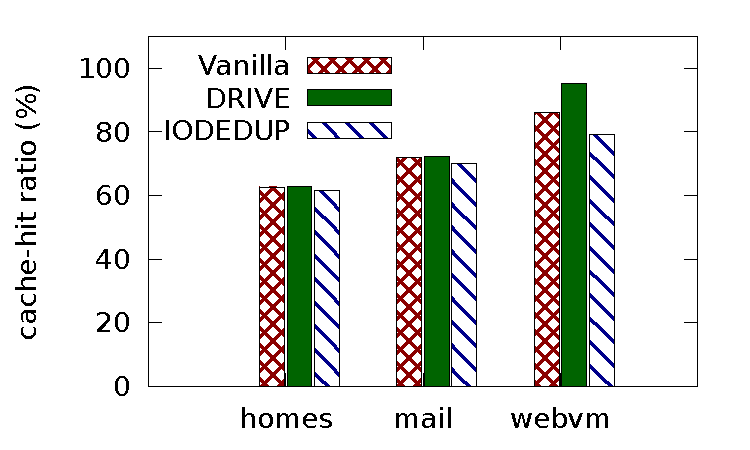
\includegraphics[scale=0.6]{confided-figures/cache-hit-rate/reads-writes/eval-reads-n-writes.pdf}} \hfill
	\subfloat[Disk read reduction]{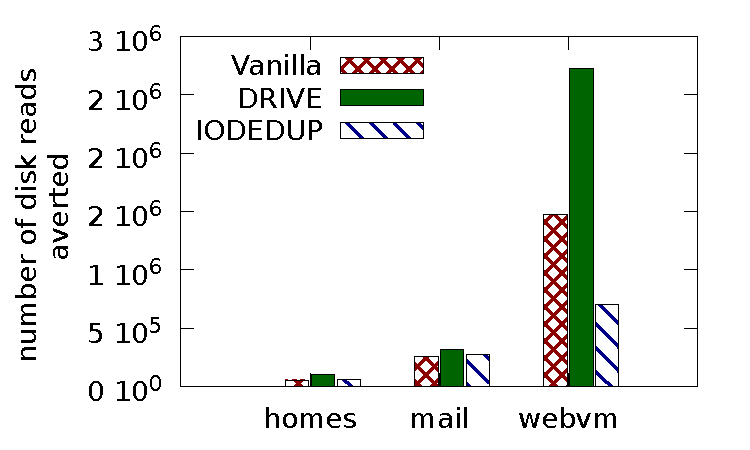
\includegraphics[scale=0.6]{confided-figures/disk-fetches-averted/reads-writes/readsaverted-reads-n-writes.pdf}}
%	\subfloat[]{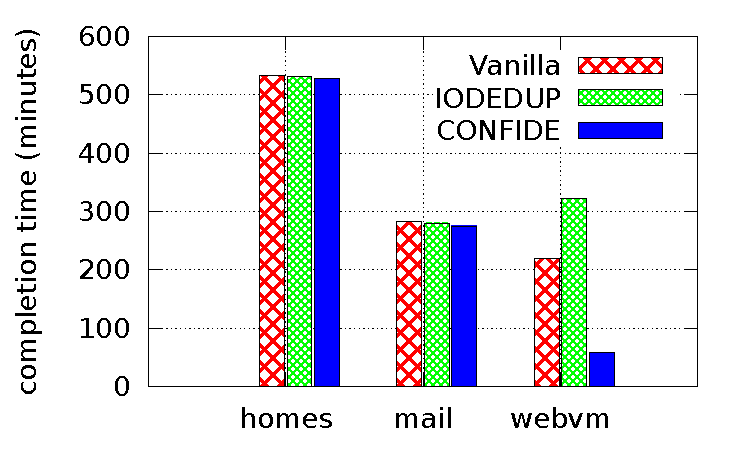
\includegraphics[scale=0.45]{confided-figures/total-completion-time/reads-writes/completiontime-reads-n-writes.pdf}}
	\caption{Comparison based on \textit{measured metrics} for read/write traces}
	\label{fig:eval-read-write-perf-a}
\end{figure}

	\vspace{-0.2in}
\begin{figure}[t]
% 	\centering
	\subfloat[Read response latency]{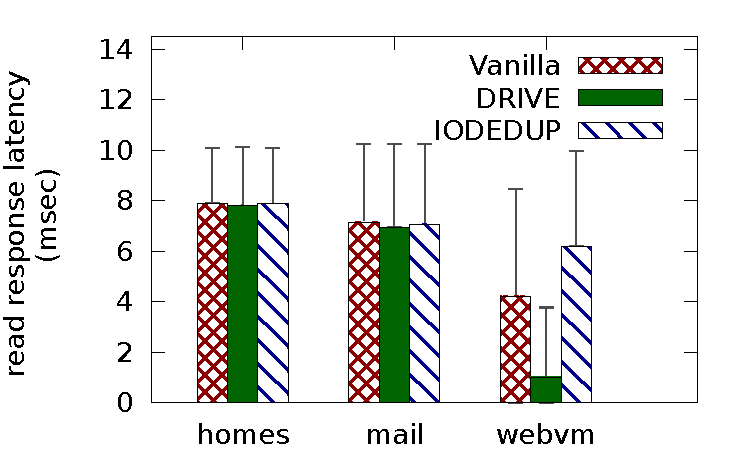
\includegraphics[scale=0.6]{confided-figures/io-latency-normal/reads-writes/iolatency-reads-n-writes.pdf}} \hfill
	\subfloat[Read response throughput]{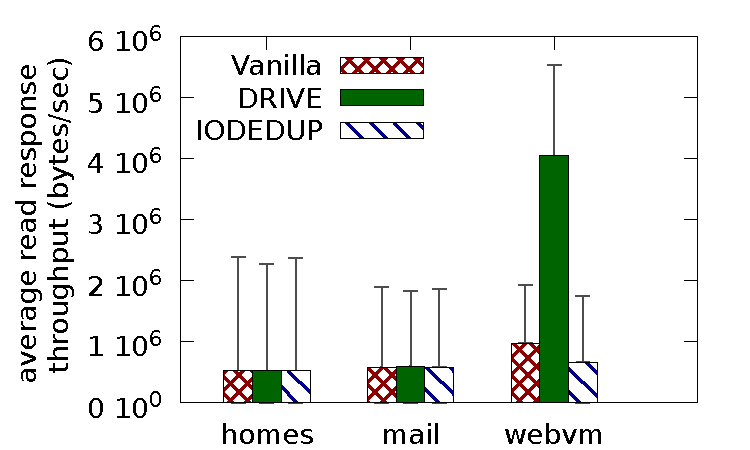
\includegraphics[scale=0.6]{confided-figures/io-latency-normal/reads-writes/iothroughput-reads-n-writes.pdf}}
	\caption{Comparison based on \textit{derived metrics} for read/write traces}
	\label{fig:eval-read-write-perf-b}
\end{figure}


\subsection{Evaluating performance with read/write workloads}
In this experiment, we replay both read and write requests of the traces
in our simulation module, and count the number of cache-hits incurred.
Note that, the number of cache hits
incurred exclusively for read requests is equivalent to the number of
disk reads reduced.
With this in mind, we report two variations of the cache hits 
metric: (i)~cache hit ratio, and (ii)~number of disk reads reduced.
The difference between these two metrics is that even though the cache 
experiences churn due to both read and write requests, the former metric
reflects all cache-hits whereas the latter metric reflects the cache-hits
occurring on account of read requests only.
We use a total memory size of 1GB, and consider 10\%
as content-cache size for IODEDUP in all further experiments.

Fig.~\ref{fig:eval-read-write-perf-a}(a) presents the cache hit ratio 
per workload for Vanilla, IODEDUP and DRIVE. 
%It can be observed that 
Whereas IODEDUP performs slightly worse on 
occasion, DRIVE always performs equal or better than Vanilla.
For example, with \textit{webvm} workload, DRIVE has higher cache-hit
ratios than both Vanilla and IODEDUP, 10\% and 20\% better, respectively.
Fig.~\ref{fig:eval-read-write-perf-a}(b) presents the number of ``disk 
reads reduced'' and it shows that DRIVE performs significantly
better at this metric, with nearly 85\% improvement over Vanilla, and
a %whopping 
2.8$\times$ improvement over IODEDUP.
%Further, Fig.~\ref{fig:eval-read-write-perf}(c) shows the total completion
%time for each trace, assuming continuous replay. The latencies for 
%cache-read, cache-write and disk-read operations are assumed to be
%1$\mu$s, 1$\mu$s and 8ms, respectively~\cite{gustavo-blogpost}.
%We can see that DRIVE achieves maximum performance improvement for
%the \textit{webvm} workload, and reduces the total completion time
%to 26\% and 18\% of Vanilla and IODEDUP completion times, respectively.
As observed earlier, the \textit{webvm} trace has the highest amount
of content deduplication, and hence benefits the most from our I/O 
reduction techniques. Thus, given any disk access pattern with
significant content similarity across blocks, our system can harness the
similarity to improve host cache performance.

Fig.~\ref{fig:eval-read-write-perf-b}(a) shows the average of read
response latencies for each trace, with the standard deviation plotted
as yerrorbars. Mean cache-read and disk-read latencies are assumed as
230ns and 8ms, respectively~\cite{gustavo-blogpost}, and individual request
cache-read and disk-read latencies were sampled from normal 
distributions.
%distribution to populate individual cache-read and disk-read latencies.
Owing to the greater reduction in number of disk reads achieved by DRIVE, 
the average read response latency is lower than
Vanilla and IODEDUP. Consequently, the average read response throughput
is higher using DRIVE, as shown in Fig.~\ref{fig:eval-read-write-perf-b}(b).

\begin{figure}
	\centering
	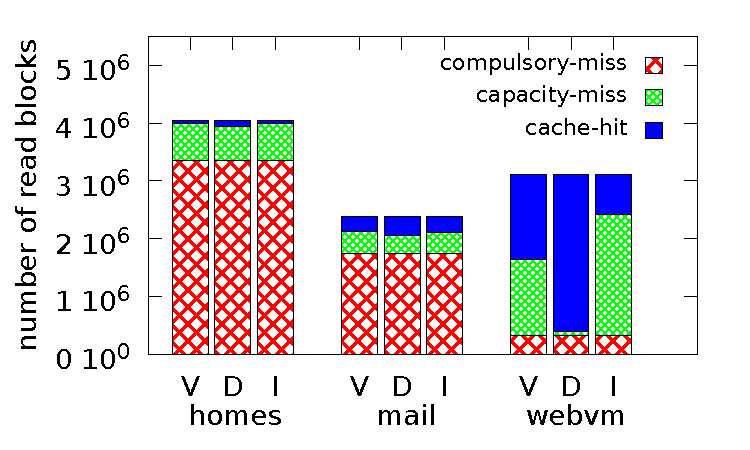
\includegraphics[scale=0.65]{confided-figures/read-response-distrib/reads-writes/read-response-distrib-reads-n-writes.pdf}
	\caption{Classification of read responses in Vanilla Vs IODEDUP Vs DRIVE for the \textit{homes}, \textit{mail} and \textit{webvm} read/write traces.}
	\label{fig:eval-read-write-perf-c}
\end{figure}


In the operation of any cache,
the first read request for every block would certainly result in a 
cache-miss. Such misses are referred as \textit{compulsory misses}
(or \textit{primary misses}),
and their number is equal to the number of different block addresses
accessed in the trace. Remaining requests in the trace would
be serviced from either cache (if present) or disk (if evicted from 
cache). Those blocks that are fetched from disk, after having been
evicted from cache at least once, are referred as \textit{capacity misses}
(or \textit{secondary misses}). 
Our performance comparison is based on reduction in number of 
capacity misses, and increase in number of cache hits.

%Fig.~\ref{fig:read-response-distrib} presents a classification
Fig.~\ref{fig:eval-read-write-perf-c} presents a classification
of the total number of read requests into \textit{compulsory misses},
\textit{capacity misses} and \textit{cache hits}, for each workload
under each system: V for Vanilla, C for DRIVE and I for IODEDUP.
We can see that both the \textit{homes} and \textit{mail} workloads 
have a huge number of compulsory 
misses, whereas the \textit{webvm} workload has significantly fewer. 
In terms of capacity misses for the \textit{webvm} workload, DRIVE 
succeeds in reducing the number down to 5\% compared to those incurred
by the Vanilla system.
For the \textit{homes} and \textit{mail} workloads, DRIVE enables 
only marginal performance improvement. This is because, the large
number of compulsory misses in these workloads implies that metadata 
is not available for many of the blocks being requested.
Note that, most compulsory misses occur during \textit{cache warm-up}
phase of any system. Once the cache warm-up phase is over, a majority of the
read requests would be for blocks that have been previously read or 
written. Hence, performance of DRIVE system will only improve.

\subsection{Content deduplication in host cache}
\begin{figure}[]
\centering
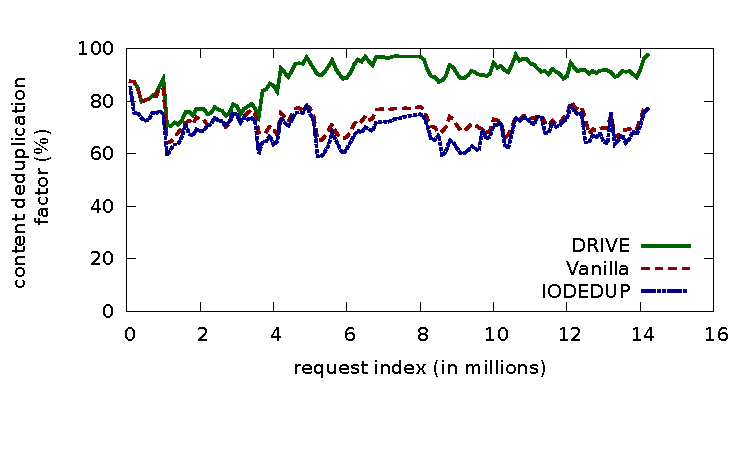
\includegraphics[scale=1]{confided-figures/contentdedup-factor/contentdedupfactor.pdf}
\vspace{-0.4in}
\caption{Content deduplication factor of page cache upon \textit{webvm} trace.}
\label{fig:contentdedup-factor-timeseries}
%\vspace{-0.1in}
\end{figure}

We claim that the DRIVE system 
effectively manipulates the host page-cache as a content-deduplicated
cache. We define 
\textit{content deduplication factor} as the ratio of number of unique
content blocks to the total number of blocks in cache. Thus, higher the
content deduplication factor, better is the efficiency of the cache.
Fig.~\ref{fig:contentdedup-factor-timeseries} shows the variation in
content deduplication factor, as each request of the \textit{webvm}
trace is replayed. It can be seen that the DRIVE system achieves
significantly higher content deduplication factor than both the 
Vanilla and IODEDUP systems. Note that, 100\% content deduplication 
of page cache can not be achieved because of the compulsory misses
incurred during cache-warmup, as well as the cache dirtying due to 
write requests. However, DRIVE attains a high 
content deduplication factor of up to 97\%, and this is the reason for 
the significant performance improvement achieved by DRIVE.

%Commented for camera-ready%%%%%%%%%%%%%%%%%%%%% BEGIN
%\subsection{Evaluating performance with read-only and write-only workloads}
%In this experiment, we wish to compare the DRIVE system against the 
%I/O Deduplication module implementation as well as the Vanilla system
%for read-only and write-only request traces. 
%We use the same traces as 
%mentioned above,
%however for read-only replay, the write requests are ignored 
%whereas for write-only replay, the read requests are ignored. 
%This is so that only read requests or only write requests are 
%replayed and affect the block-cache and/or content-cache behaviour, for
%this experiment. 
%
%%Commented for camera-ready
%\begin{figure}
%% 	\centering
%	\subfloat[Read-only]{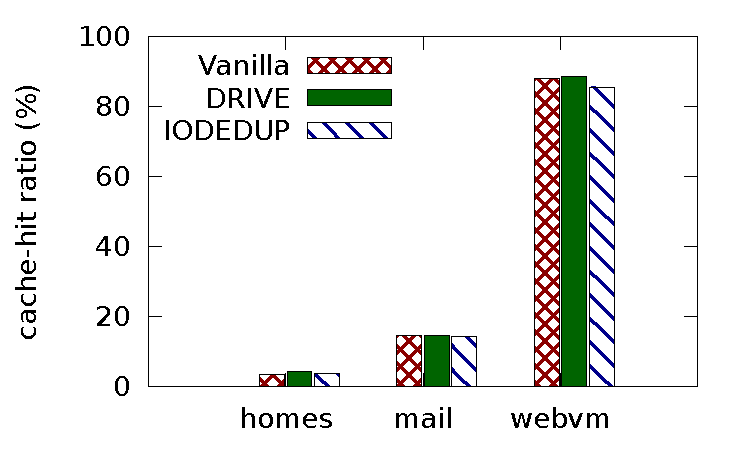
\includegraphics[scale=0.6]{confided-figures/cache-hit-rate/reads/eval-reads.pdf}} \hfill
%	\subfloat[Write-only]{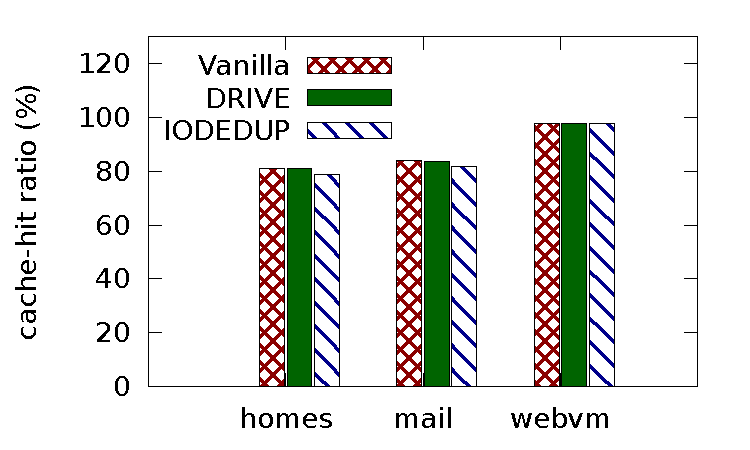
\includegraphics[scale=0.6]{confided-figures/cache-hit-rate/writes/eval-writes.pdf}} 
%%	 \vspace{-0.05in}
%	\caption{Cache-hit ratios for Vanilla Vs IODEDUP Vs DRIVE for \textit{homes}, \textit{mail} and \textit{webvm} read-only and write-only traces.}
%	\label{fig:eval-read-only-write-only-perf}
%\end{figure}
%
%%Commented for camera-ready
%Fig.~\ref{fig:eval-read-only-write-only-perf}(a) shows the cache hit 
%ratio per workload
%for the three systems\textemdash{}Vanilla, IODEDUP and DRIVE for read-only
%replay of the traces. As can seen, IODEDUP performs better than
%Vanilla for \textit{homes} and \textit{mail} workloads, but is worse
%for \textit{webvm} workload. In contrast, DRIVE cache-hit ratio is 
%always equal or better than Vanilla for all workloads' read-only requests
%streams, for example, up to
%19\% better than Vanilla and 10\% better than IODEDUP for \textit{homes}
%workload.
%Fig.~\ref{fig:eval-read-only-write-only-perf}(b) shows the corresponding 
%cache hit ratios for the write-only replay of the traces. 
%IODEDUP has marginally lower
%cache-hit ratios than Vanilla for all three workloads. However, DRIVE
%performs much better for write-only request streams, and performs 
%at least as well as Vanilla.
%Commented for camera-ready%%%%%%%%%%%%%%%%%%%%% END

\subsection{Identifying similarity in multiple virtual machines}
To simulate the scenario of multi-VM workloads being executed on a
virtualized host, we aggregated the two three-week long traces of
\textit{homes} and \textit{webvm} workloads in timestamp order. We 
performed a read/write replay of the aggregate trace and compare
cache-hit ratios, disk reads reduced and read response latencies for
Vanilla, DRIVE and IODEDUP. 

\begin{table}[h]
\caption{Performance for aggregated trace replay}
\label{tab:aggregate-hw}
\centering
\begin{tabular}{|c|c|c|c|} \hline
\textbf{Scheme} & \textbf{Cache-hit} & \textbf{Disk reads} & \textbf{Avg. read}  \\
\textbf{} & \textbf{ratio (\%)} & \textbf{reduced(\%)} & \textbf{response latency (msec)}  \\ \hline
%\textbf{} & \textbf{} & \textbf{} & \textbf{latency} \\ \hline
\textit{Vanilla} & 61.2 & 1.6 & 7.9 \\ \hline
\textit{DRIVE} & 67.6 & 18.5 & 6.5 \\ \hline
\textit{IODEDUP} & 62.4 & 4.3  & 7.7 \\ \hline
\end{tabular}
%\vspace{-0.15in}
\end{table}

The performance metrics are tabulated in 
Table~\ref{tab:aggregate-hw} and show that although the cache-hit ratios
are comparable in all three schemes (DRIVE is highest nevertheless),
there is a huge margin in percentage of disk reads reduced. DRIVE system
averts 18\% disk reads as compared to 1.6\% of Vanilla and 4.3\% of IODEDUP.
Decrease in number of disk reads results in a lower average 
read response latency, with 6.5ms for DRIVE as compared to
7.9ms and 7.7ms for Vanilla and IODEDUP, respectively.
Fig.~\ref{fig:aggregate-hw-time-series} plots the read response throughput
per hour, assuming continuous replay of read requests in the aggregated trace.
We can see that DRIVE produces more number of responses per hour in the 4th,
5th, 6th hours and so on, hence resulting in an earlier completion than
Vanilla or IODEDUP replays. Notably, in hour 13, DRIVE finishes almost
double the number of read requests as Vanilla and IODEDUP.

\begin{figure}[h]
\centering
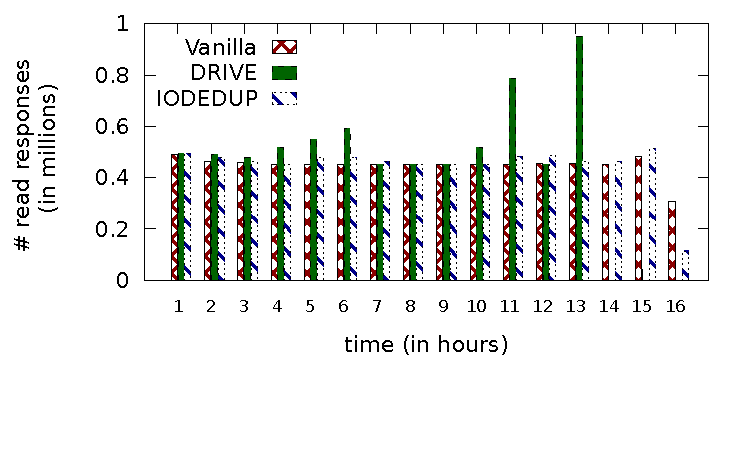
\includegraphics[scale=0.90]{confided-figures/aggregate-hw-replay/reads-writes/timeseriesperf-hour.pdf}
\vspace{-0.6in}
\caption{Read response throughput for the aggregated trace.}
\label{fig:aggregate-hw-time-series}
%\vspace{-0.1in}
\end{figure}

\subsection{Evaluating impact of write-intensivity factor}
The presence of write requests
demands continuous metadata updates and also causes cache churn, which
results in lowered cache hit performance for read requests. Hence, 
it is important to study effectiveness of cache manipulation with
write-intensive workloads as well. 

\begin{figure}[h]
\centering
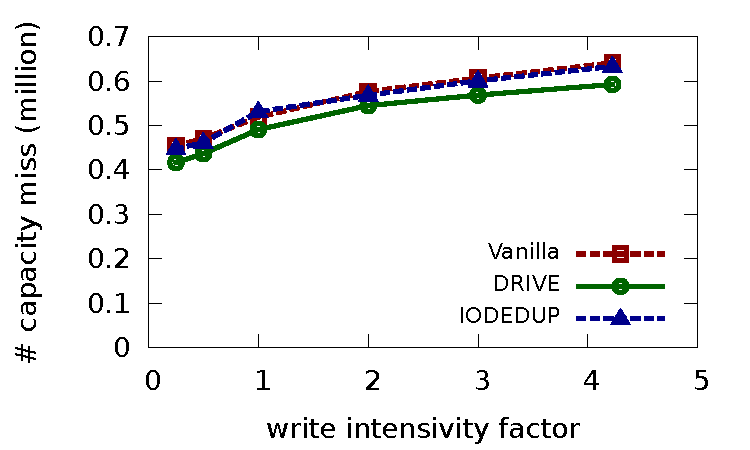
\includegraphics[scale=0.78]{confided-figures/write-intensivity-factor/reads-writes/homes-wif.pdf}
%\vspace{-0.15in}
\caption{Impact of write-intensivity factor for the \textit{homes} workload.}
\label{fig:wif-impact}
%\vspace{-0.2in}
\end{figure}

In this experiment, we generated trace-snippets with various 
write-intensivity
levels using the \textit{homes} workload as base trace, and
probabilistically sampling write requests. The write-intensivity of the
original \textit{homes} trace is 4.2, and we generated trace-snippets
with varying write-intensivity levels like 0.25, 0.5, 1, 2 and 3, and
performed trace-based replay. 
As seen in Fig.~\ref{fig:wif-impact}, as the write-intensivity level
increases from 0.25 to 4.2, the difference in
number of capacity misses between Vanilla and DRIVE increases. 
This implies that even as the write-intensivity factor increases, DRIVE is 
able to convert higher number of capacity misses into cache-hits. 
Thus, DRIVE performs well even with write-intensive workloads.

